\label{testbeamreq}
\subsection{Particle beam requirements}
The requested beam parameters are driven by the requirement that the results from the CERN test beam should be directly applicable to the future large underground single-phase LAr detector with minimal extrapolation. The CERN test beam data will be used to evaluate the detector performance, to understand the various physics systematic effects, and to provide ``neutrino-like'' data for event reconstruction studies. To satisfy the requirement, the beam parameters must span a broad range of particle spectrum that are expected in the future neutrino experiment. The particle beam composition should consist of electrons, muons, and hadron beams that are charge-selected. The expected momentum distributions for secondary particles from neutrino interactions are shown in Figure~\ref{fig:particle_momenta}. There is a large spread in the momentum distribution with most particles peaked near 200 MeV/c. To cover the momentum range of interest, the momentum of the test beam should step from 0.2 GeV/c up to 10 GeV/c. 

The maximum electron drift time in the TPC is about 2.2 ms. In order to minimize pile-up in the TPC, the planned beam rate should be around 200 Hz.  The DUNE-PT has two drift volumes separated by a passive cathode plane.
It is desirable to aim the particle beam such that a large fraction of the lower energy hadronic showers are mostly contained in one drift 
volume to minimize uncertainties due to the passing of inactive detector materials.

The nominal plan is to have the beam enter the cryostat slightly downward at an angle of about 6 degrees. This angle will roughly match the angle at which the neutrino beam enters the liquid argon cryostat at the far detector for the DUNE experiment. Along the horizontal plane, the beam should enter the cryostat with an angle of about 10 degrees to avoid pointing the beam perpendicular to the electron drift in the TPC.  
Events with the latter orientation would introduce larger reconstruction ambiguities. 
We also plan to take some data with the beam entering a different region of the TPC, and may include some data with particles crossing one drift volume to the next.  The summary of the beam requirements are shown in Table~\ref{table:beamspecs}.
%The two beam entry angles and positions with respect to the LAr cryostat are shown in Figures \ref{fig:BP_SideView} and \ref{fig:BP_TopView}. 

%\begin{figure}[h!]
%  \centering
%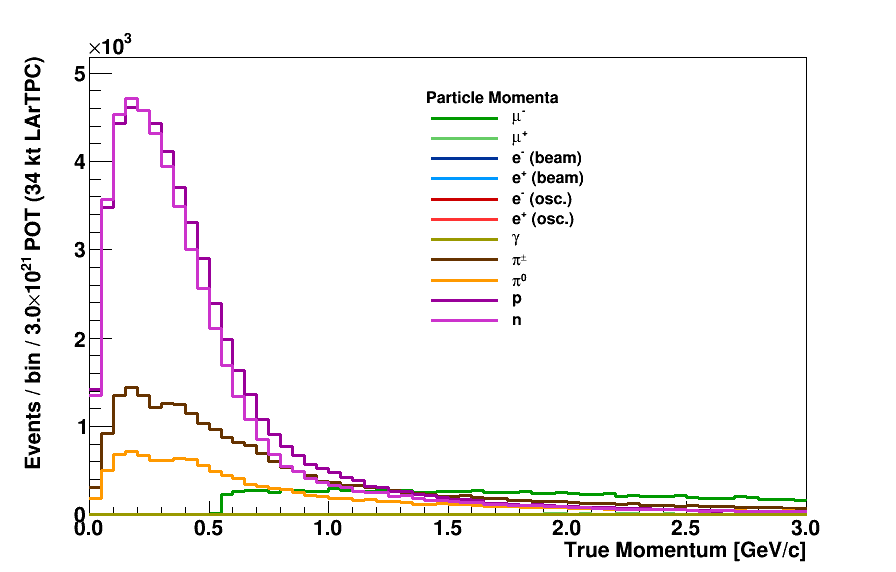
\includegraphics[scale=0.5]{figures/True_Momenta_per_Particle.png}
%  \caption{Particle momenta distributions for particles coming from all fluxes ($\nu_e$, $\nu_\mu$, $\bar \nu_e$ and $\bar \nu_\mu$) at both near and far detector locations.  }
%  \label{fig:particle_momentav2}
%\end{figure}

%\begin{figure}[h]
%  \centering
%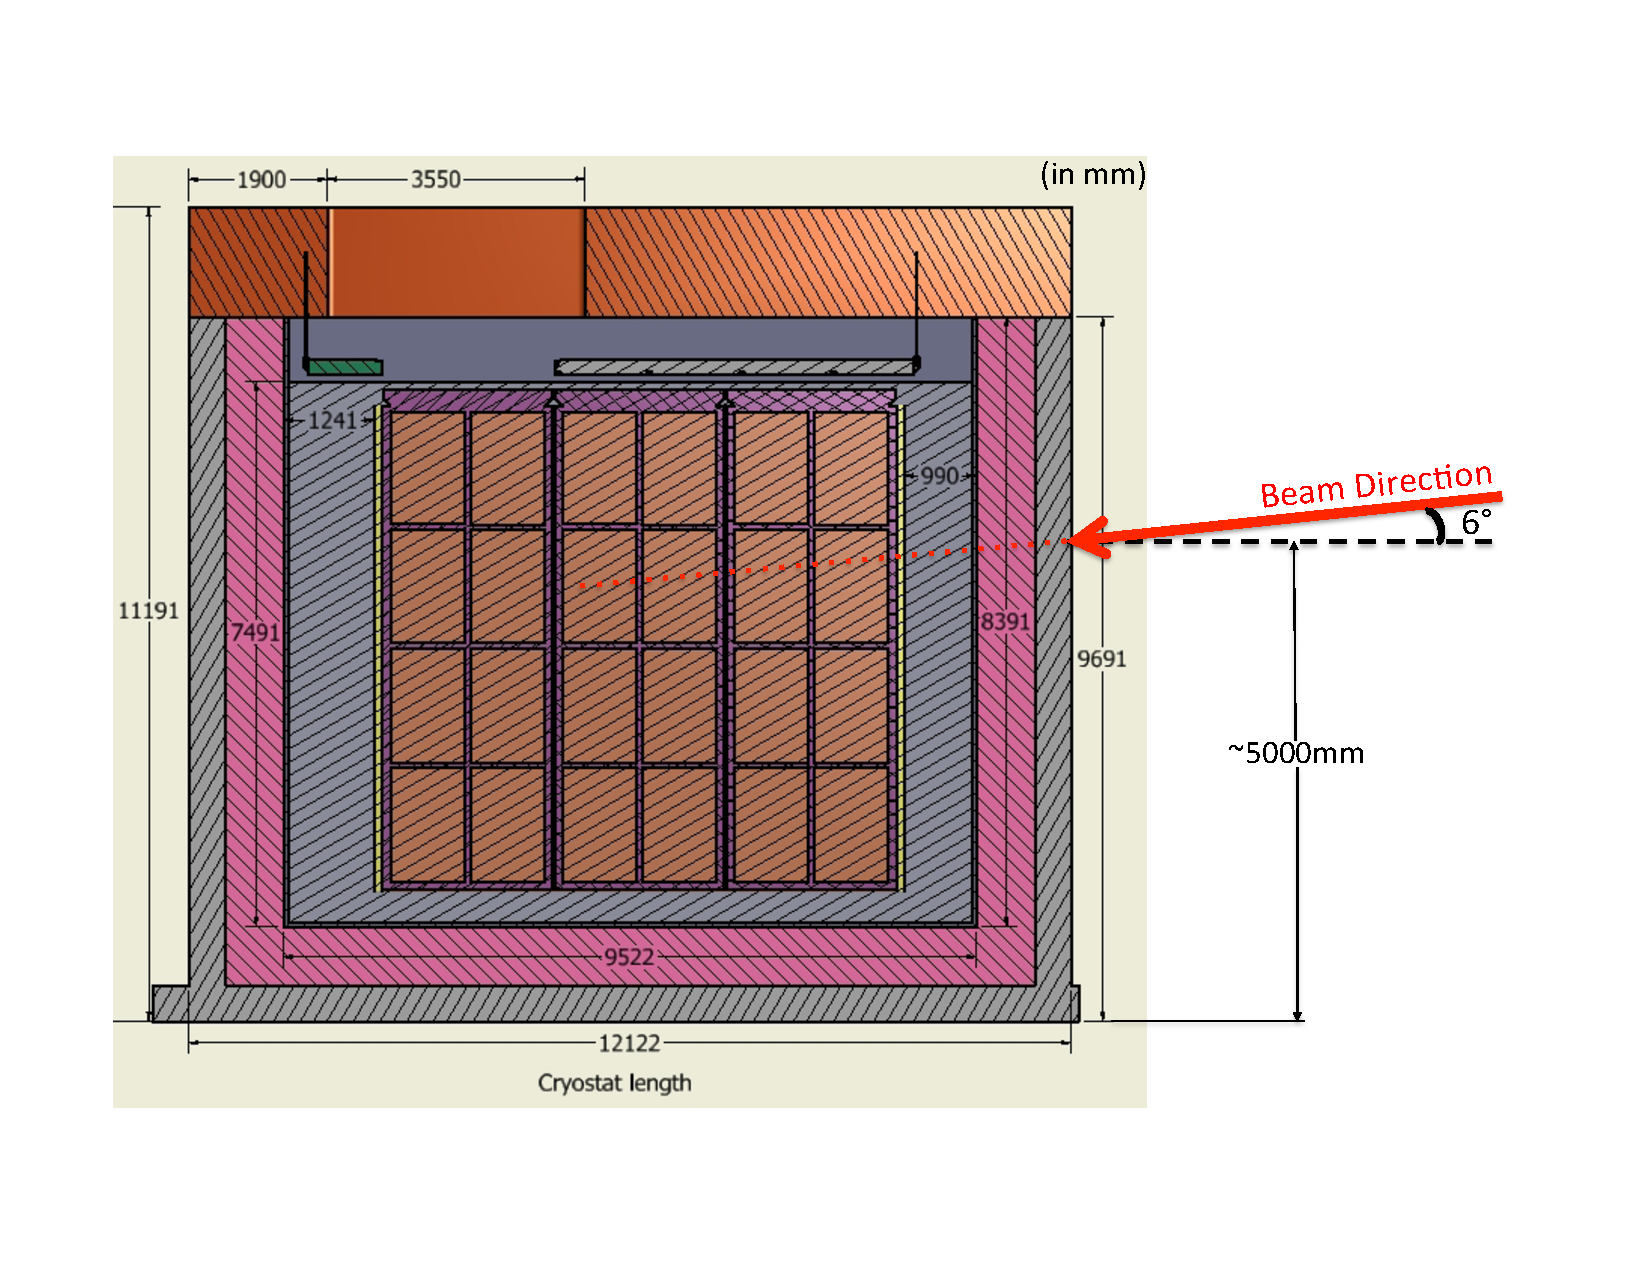
\includegraphics[scale=0.6]{figures/BeamPos_SideView.pdf}
%  \caption{Side view: beam enters the cryostat slightly downward with a dip angle of 6 degrees.  }
%  \label{fig:BP_SideView}
%\end{figure}
%
%\begin{figure}[h]
%  \centering
%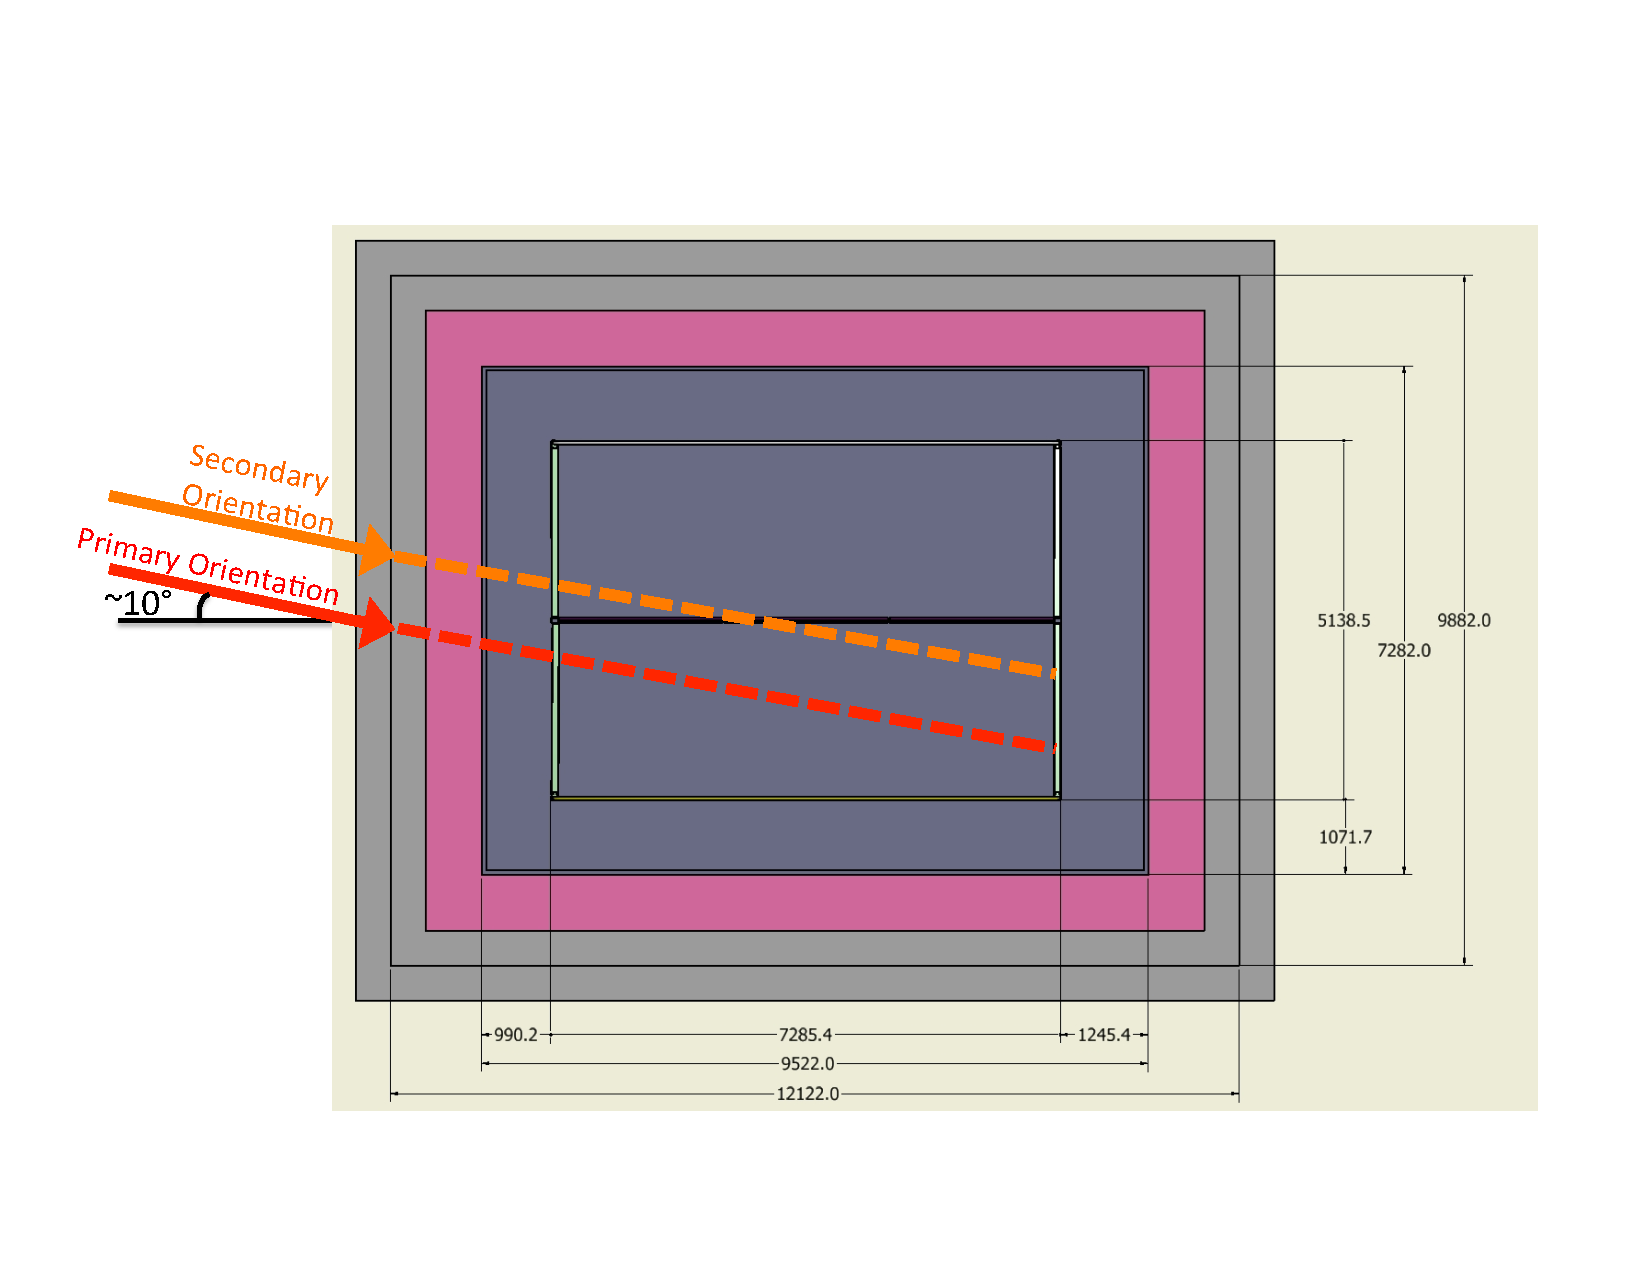
\includegraphics[scale=0.6]{figures/BeamPos_TopView.pdf}
%  \caption{Top view: beam enters the cryostat with an entry angle of about 10 degrees along the horizontal plane. The primary orientation sends the particle beam into one TPC drift volume. The secondary orientation sends the particle beam across the APA. }
%  \label{fig:BP_TopView}
%\end{figure}

\begin{table}[h]
\centering
\begin{tabular}{|c|c|}
\hline
\textbf{Parameter } & \textbf{Requirements}  \\ \hline
  Particle Types        & $e^\pm,\mu^\pm,\pi^\pm$,$K$,$p$  \\ \hline
  Momentum Range   & 0.2 - 10 GeV/$c$ \\ \hline
  Momentum Spread   & $\Delta p/p  < $5 \% \\
  & (limited by the aperture of the magnets)  \\ \hline
  Transverse Beam Size   & RMS(x,y) $\approx$ 10 cm  \\
  & (At the entrance face of the LAr cryostat) \\ \hline
  Beam Divergence & tbd   \\ \hline
  Beam Angle &  $\approx$10$^{\circ}$ \\
  (horizontal plane) &  (w.r.t. the long axis of the cryostat)\\ \hline
  Beam Dip Angle &  $\approx$6$^\circ$ (downward from horizontal)   \\ 
  (vertical plane) &  \\ \hline
  Beam Entrance Position & Multiple beam windows    \\ \hline
  Rates & 200 Hz (maximum)    \\ \hline
\end{tabular}
\caption{Particle beam requirements.}
\label{table:beamspecs}
\end{table}

\subsection{EHN1 H4ext beamline and beam instrumentation}
The H4ext is an extension of the existing H4 beamline in Experimental Hall North 1 (EHN1).  To produce particles in the momentum range of interest, a 60-80 GeV/c pion beam from the T2 target is used to generate tertiary beams. The tertiary particles are momentum and charge-selected and transported down H4ext beamline to the experimental area. A conceptual layout of the H4ext beamline is shown in Fig.~\ref{fig:H4extPrelim}.  The top plot in Fig.~\ref{fig:H4extPrelim} is the bird's eye view and the bottom plot is the side view of the beam line layout.
%In the Figure, the cryostat for this proposal is located at the lower right hand corner of the plot (in the H4 beam line). The cryostat in the H2 beam line is for the WA105 Collaboration.

\begin{figure}[h]
  \centering
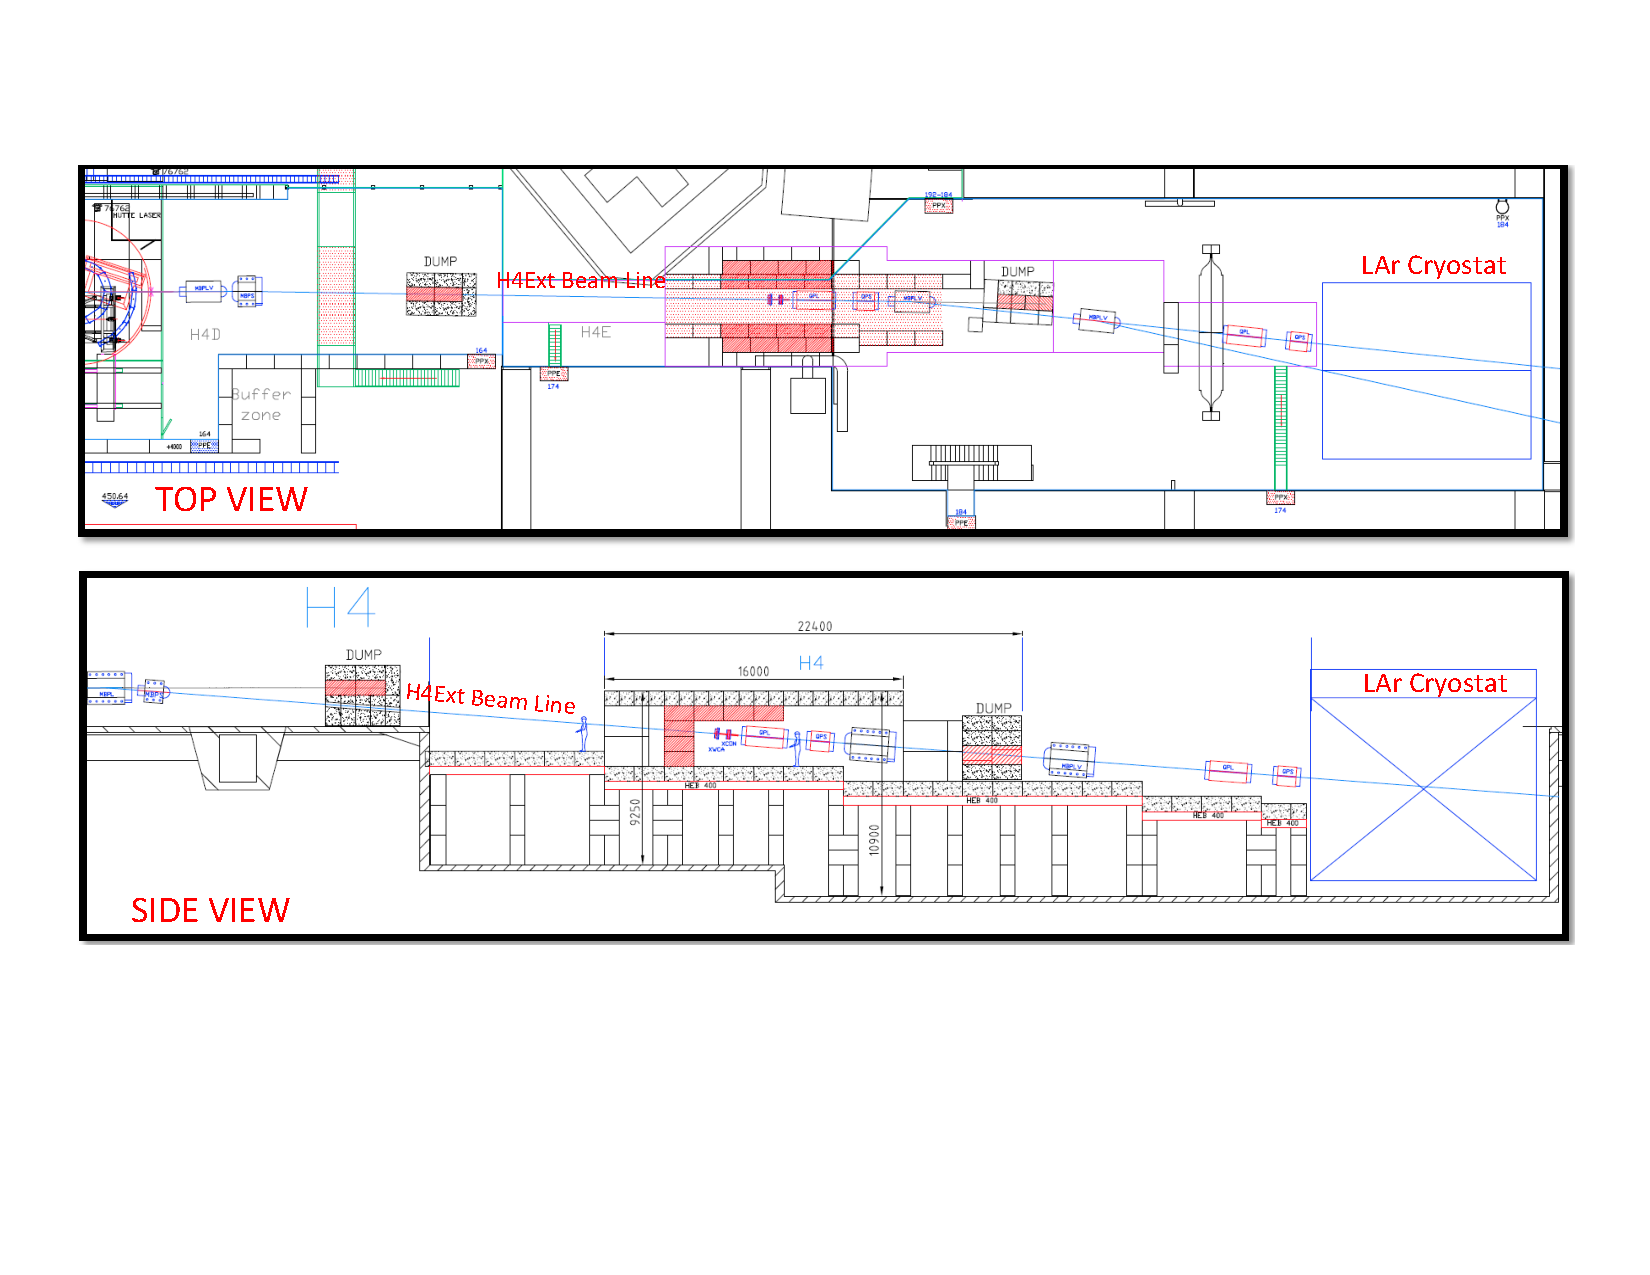
\includegraphics[scale=0.62]{figures/EHN1_H4ext.pdf}
  \caption{A conceptual layout of the H4ext beamline. The top plot is the bird's eye view and the bottom plot is the side view of the H4ext beam line in EHN1. The liquid argon cryostat for this proposal is the rectangular box in the right hand corner of both plots.  The beam nominally enters the TPC at an angle of about 10$^\circ$ horizontally (top plot). On the vertical plane (bottom plot), the beam enters the cryostat downward with an angle of about 6$^\circ$. Multiple beam windows will be installed on the upstream wall of the cryostat to allow the beam to enter the TPC from different positions and angles.}
  \label{fig:H4extPrelim}
\end{figure}

%\subsubsection{Beam Optics}
%[Waiting for inputs from Ilias]

%\subsection{Beam Instrumentation}
\label{beaminstrument}
Beam instrumentation provides important information about the characteristics of the beam. It is expected that a series of detectors will be installed along the beam line to measure the particle momentum, identify particle type, and track the particle trajectory.

\subsubsection{Beam position detector}
The beam position detector measures the positions of the particle as it traverses the detector. Two detector technologies are under considerations: wire chambers and scintillating fiber trackers. For the nominal setup, one beam position detector is installed upstream and another one downstream of the last bending magnet. This pair provides additional momentum information about the particles as well as the first set of position measurements. Without tracking information, the momentum spread of the beam is expected to be at around 5\% based on the acceptance of the dipole magnets. With additional tracking information, we are likely to be able to measure the momentum of the individual particles to close to one percent level. A third beam position detector is placed right in front of the beam window on the cryostat wall to provide the last position information before the beam enters the cryostat.

\subsubsection{Particle identification}
In order to have good particle identification over large momentum range, two independent particle identification systems are needed in the beamline. The Time-of-Flight system will be used to cover the lower momentum range while a Threshold Cherenkov detector will be tuned for higher momentum particles. We will require $\geq$ 3$\sigma$ $K$/$\pi$ separation for momentum range from 0.2 to a few GeV/c. Work is in progress to better define the beamline layout to meet the requirements.

\subsubsection{Muon beam halo counters}
The muon beam halo counters is a set of detectors (e.g. plastic scintillator paddles) surrounding the beamline. The main purpose is to tag particles (primarily muons from the upstream production target) that are outside of the beam axis, but may potentially enter the TPC volume. The counter information is used to either veto or simply flag these class of events. The Muon Beam Halo counter can be a subset of the cosmic muon veto system. 

%\subsection{Beam Window on LAr Cryostat}
%This section could be absorbed into the cryostat chapter.


\subsection{Beam rates and run plan}
At the time of this proposal, the beamline design has not been finalized. To estimate the beam rates, we use inputs from a generic target simulation based on 100k 80 GeV $\pi^+$ beam on 15 cm copper target. This $\pi^+$ rate is roughly equivalent to 10\% of a typical SPS spill. The distributions of the tertiary particles from the copper target are shown in Fig.~\ref{fig:PionOnCuTarget}. The figure on the left is for postively charged and the figure on the right is for negatively charged tertiary particles. 

\begin{figure}[tbh]
  \centering
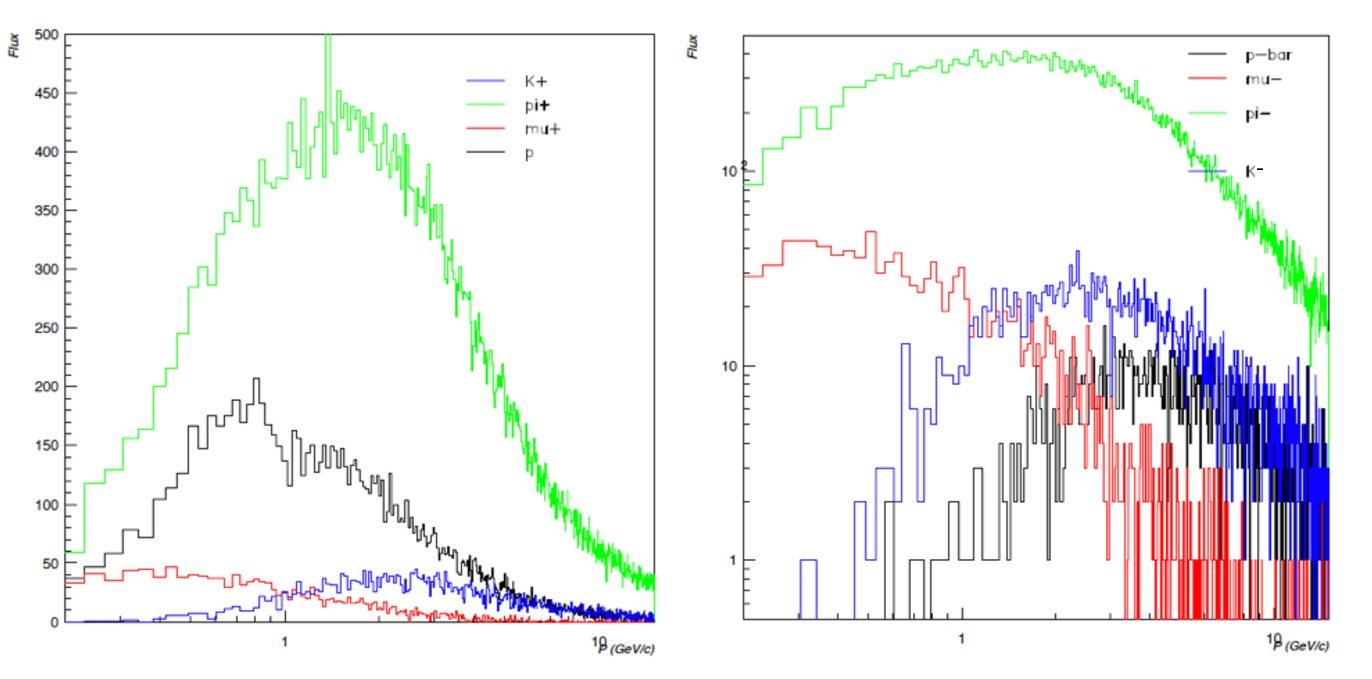
\includegraphics[scale=0.47]{figures/80GeVPion-15cmCuTarget.jpg}
  \caption{Simulated flux of charged secondary particles resulting from 100k $\pi^+$ each with an energy of 80~GeV impinging on a 15 cm copper target. The figure on the left is for positively charged and the figure on the right is for negatively charged secondary particles.}
\label{fig:PionOnCuTarget}
\end{figure}

To formulate a preliminary beam time request, we assume the hadron beam rates and spectrum as given in Fig.~\ref{fig:PionOnCuTarget}. For the beam rate estimates, we account for particle decays assuming the distance from the secondary target to the cryostat to be 30 m. A significant fraction of pions and kaons below 1 GeV/c decay before reaching the liquid argon cryostat. In addition, we also assume the data taking efficiency to be about 50\%. For the electron sample, we expect a different optimized beamline setup to produce a pure electron beam with a flux of about 200 Hz. A preliminary run plan for one configuration is shown in Table~\ref{tab:RunPlan}. 
%
\begin{table}[p]
\centering
\rowcolors{0}{gray!30}{gray!30}
\begin{tabular}{|c|c|c|c|c|c|c|}
\hline
\multicolumn{7}{|c|}{\bf Positive Sample} \\ \hline
\bf $P$ & \bf $\#$ of Spills & \bf Time & \bf $\#$ of $\pi^+$ & \bf$\#$ of $\mu^+$ & \bf$\#$ of $K^+$ & \bf$\#$ of p \\ 
\bf (GeV)& & \bf (hours) & & & & \\ \hline
\hiderowcolors
0.2&900 &11&\textcolor{red}{\bf 15k} &180k&$\approx$0&160k\\ 
0.3&200 &3 &\textcolor{red}{\bf 15k} &30k &$\approx$0&50k \\
0.4&150 &\textcolor{red}{\bf 2} &22k &18k &$\approx$0&32k \\ 
0.5&150 &\textcolor{red}{\bf 2} &26k &12k &$\approx$0&38k \\
0.7&150 &\textcolor{red}{\bf 2} &40k &10k &$\approx$0&45k \\
1  &350 &4 &120k&\textcolor{red}{\bf 10k} &$\approx$0&65k \\
2  &600 &8 &320k&\textcolor{red}{\bf 10k} &3k        &130k\\
3  &500 &6 &290k &\textcolor{red}{\bf 5k} &7k        &70k \\
5  &1800&23& 1M &\textcolor{red}{\bf 5k}  &5k        &270k\\
7  &1200&15&660k&\textcolor{red}{\bf 6k}  &3k        &120k\\ \hline
Total &6000&76&2.5M  & 286k  &18k   & 1M\\
\hline \hline
\multicolumn{7}{|c|}{\bf Negative Sample} \\ \hline
\showrowcolors 
\bf $P$ & \bf $\#$ of Spills & \bf Time & 
\multicolumn{2}{|>{\columncolor[gray]{0.83}}c|}{\bf $\#$ of $\pi^-$ }& 
\multicolumn{2}{|>{\columncolor[gray]{0.83}}c|}{\bf$\#$ of $\mu^-$ } \\ 
\bf (GeV)& & \bf (hours) & 
\multicolumn{2}{|>{\columncolor[gray]{0.83}}c|}{}& 
\multicolumn{2}{|>{\columncolor[gray]{0.83}}c|}{} \\ \hline  
\hiderowcolors
0.2&600&8&\multicolumn{2}{|c|}{\textcolor{red}{\bf 15k}} &\multicolumn{2}{|c|}{88k}\\
0.3&200&3&\multicolumn{2}{|c|}{\textcolor{red}{\bf 15k}} &\multicolumn{2}{|c|}{30k}\\
0.4&150&\textcolor{red}{\bf 2}&\multicolumn{2}{|c|}{30k} &\multicolumn{2}{|c|}{18k}\\
0.5&150&\textcolor{red}{\bf 2}&\multicolumn{2}{|c|}{40k} &\multicolumn{2}{|c|}{13k}\\
0.7&150&\textcolor{red}{\bf 2}&\multicolumn{2}{|c|}{50k} &\multicolumn{2}{|c|}{12k}\\
1  &150&\textcolor{red}{\bf 2}&\multicolumn{2}{|c|}{70k} &\multicolumn{2}{|c|}{12k}\\
2  &200&3&\multicolumn{2}{|c|}{135k}&\multicolumn{2}{|c|}{\textcolor{red}{\bf 6k}}\\ \hline
Total  &1600&22&\multicolumn{2}{|c|}{350k}&\multicolumn{2}{|c|}{180k}\\ 
\hline 
\hline
\multicolumn{7}{|c|}{\bf Electron Sample} \\ \hline
\showrowcolors 
\multicolumn{3}{|>{\columncolor[gray]{0.83}}c|}{\bf $P$} &\bf $\#$ of Spills&\multicolumn{2}{|>{\columncolor[gray]{0.83}}c|}{\bf Time}&{\bf $\#$ of electron }\\
\multicolumn{3}{|>{\columncolor[gray]{0.83}}c|}{\bf (GeV)} & &\multicolumn{2}{|>{\columncolor[gray]{0.83}}c|}{\bf (hours)}&\\
\hline
\hiderowcolors
\multicolumn{3}{|c|}{0.2,0.3,0.4,0.5,0.7,1,2,3,5,7}  & 150 per bin & \multicolumn{2}{|c|}{2 hours per bin} &{140k per bin} \\ \hline
\multicolumn{3}{|c|}{Total}  & 1500 & \multicolumn{2}{|c|}{20} &{1.4M} \\ \hline
\end{tabular}
\caption{A preliminary run plan for one beam angle and position. The number of spills needed for a given momentum bin is driven by the samples highlighted in red or by the requirement of at least 150 spills per momentum bin.}
\label{tab:RunPlan}
\end{table}
The number of spills needed for each momentum bin is driven by the samples highlighted in red. The minimum beam time requirement is 150 spills ($\approx$ 2 hours of beam time) per momentum bin to ensure we have sufficient data taken with stable beam running.  This proposed plan satisfies the requested samples as listed in Table~\ref{tab:runsum}, except for kaons less than 1 GeV. Most low momentum kaons produced from the secondary target decay before reaching the liquid argon cryostat. To obtain those samples, we will need to carry out extended runs and trigger exclusively on particles tagged as kaons by either the time-of-flight or the threshold Cherenkov counters.

In addition to the above samples with beam at the nominal position, we expect to take some additional data with the beam entering the TPC at different position and angles. Without a detail beamline design, there are still some uncertainties on the actual beam rates. We are working on estimating the amount of beam time required. Based on the current information that we have, the total estimated beam time needed to carry out the physics program (physics samples as listed in Table~\ref{tab:runsum}, multiple angles and beam positions, dedicated kaon runs, etc) in this proposal is in the range of 4 to 6 weeks.
 
